\section{Procedure}

\texttt{mlim} support several algorithms. These algorithms have different computational needs and \texttt{mlim} optimizes the imputation procedure without requiring excessive computational resources. These algorithms, their computational requirements, and \texttt{mlim} optimization procedure is further explained below.

\subsection{Imputation steps}

\texttt{mlim} follows three steps to carry out the imputation:

\begin{enumerate}
    \item \textbf{Preimputation} : Instead of replacing missing observations with mean or mdoe, a very fast \textbf{RF} (Random Forest) algorithm is used to carry out a primary single imputation. The imputed data will be further optimized in the following steps.
    \item \textbf{Reimputation} : The preimputed data will be reimputed with \textbf{ELNET} (default) or another algorithm. 
    \item\textbf{Postimputation} : The reimputed data can be even further optimized using a heavier algorithm that requires much more computational resources such as \textbf{GBM}, \textbf{XGB}, \textbf{DL}, or all of them via \textbf{Ensemble}. The latter trains a stacked ensemble from all of the available trained algorithms to minimize imputation error as much as possible, within the given fine-tuning time. \textbf{\color{violet}Note: Using 'Ensemble' is not recommended for general imputation practice and is intended for particular cases or smaller datasets were minimizing imputation error can make a significant difference.}
\end{enumerate}

\subsection{Preimputation, reimputation, and postimputation}

although the third step is optional. The algorithm begins with a preimputation, which is a quick imputation with Random Forest. The reason for pre-imputation is to save time on the reimputation. Therefore, instead of replacing missing observations with mean and mode and starting a slow procedure for optimizing the imputed values, a fast and efficient algorithm is used for initial imputation and then, the imputed values are optimized. For the second step, the \texttt{ELNET} algorithm is fine-tuned. Note that what makes \texttt{ELNET} slower than Random Forest is the fact that \texttt{ELNET} is being fine-tuned but the preimputation procedure is not fine-tuned and a fixed model is used for any variable, regardless of variable type or data size. 

\vspace{10pt}

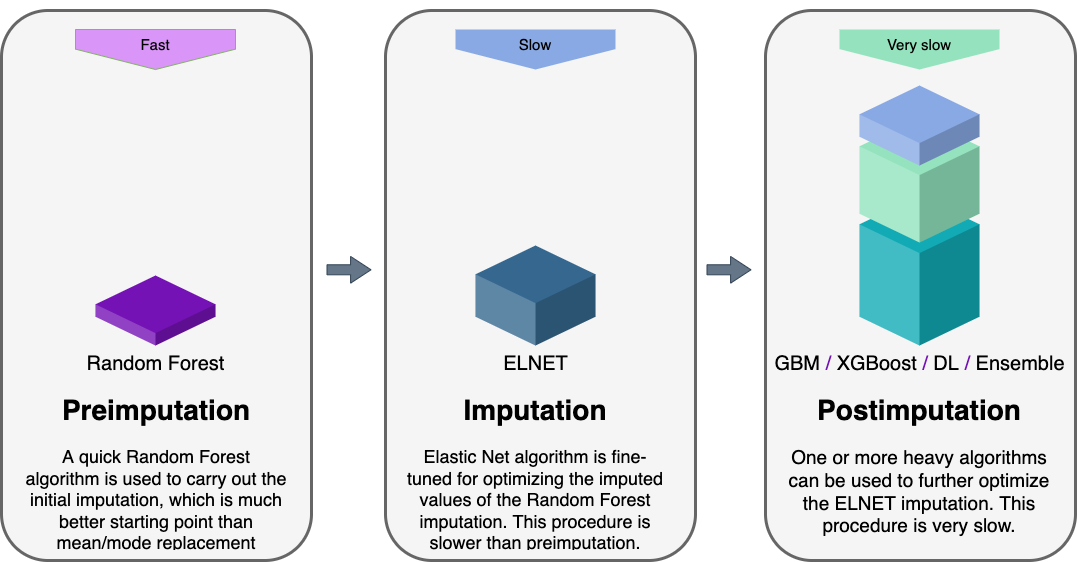
\includegraphics[scale=0.35]{figures/procedure3.png}

\subsection{Supported algorithms}

\begin{itemize}
    
    \item \textbf{\color{violet}RF} (Random Forest and Extreme Randomized Trees). This algorithm is only used in \textit{preimputation}, but it can also be used as the main imputation algorithm or \textit{postimputation} (see below for definitions)
    
    \item \textbf{\color{blue}ELNET} (Elastic Net). This is the main default imputation algorithm
    
    \item \textbf{\color{teal}GBM} (Gradient Boosting Machine).  
    \item \textbf{\color{teal}XGB} (Extreme Gradient Boosting, available in Mac OS and Linux).
    \item \textbf{\color{teal}DL} (Deep Learning).
    \item \textbf{\color{teal}Ensemble} (Stacked Ensemble, only works if other algorithms are also present).
\end{itemize}




\section{Fast optimization with \texttt{ELNET}}

As noted earlier, \texttt{mlim} carries out optimization process on preimputed data. The fastest algorithm for optimizing imputed missing data is \texttt{ELNET}, which is also more fair towards imbalanced data and categories with lower prevalence. As shown in the figures below, \texttt{ELNET} optimization already outperforms all other statistical and machine learning single or multiple imputation algorithms available in \textbf{R}. 

\hspace{-30pt}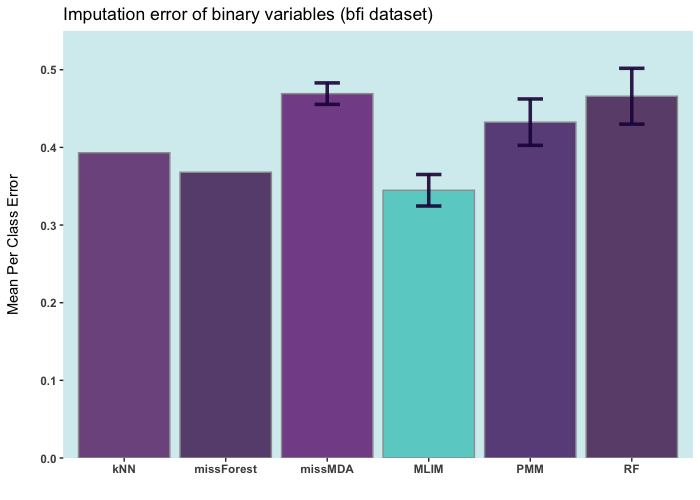
\includegraphics[scale=.3]{figures/bfi_binary_p15.png}
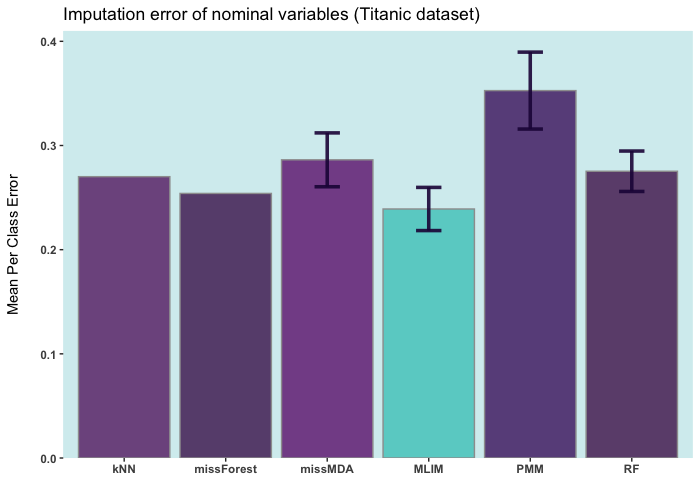
\includegraphics[scale=.3]{figures/titanic_mpce_p15.png}

\hspace{-30pt}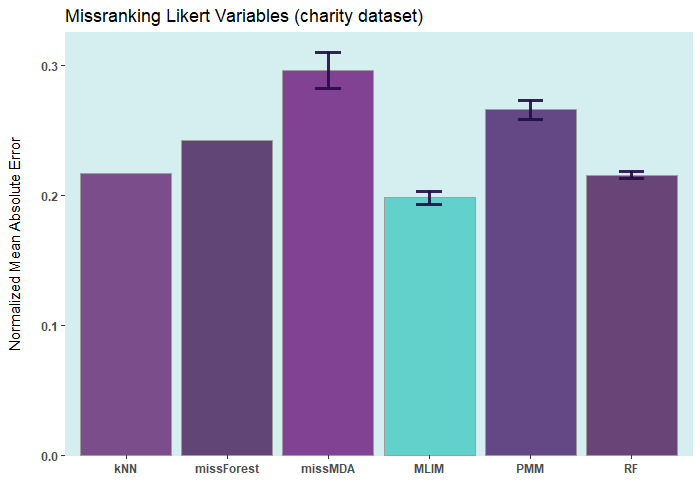
\includegraphics[scale=.4]{figures/charity.png}
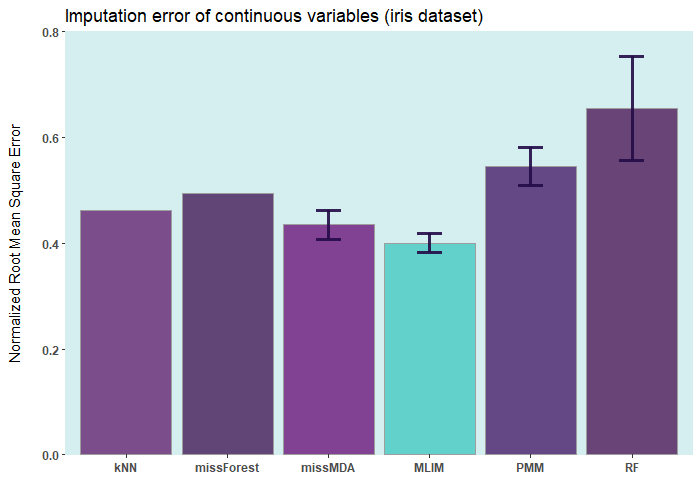
\includegraphics[scale=.4]{figures/iris_continuous_p15.png}

The analysis above uses four different datasets and adds artificial missingness at the rate of 15\% to all variables. Then several famous \textbf{R} algorithms are used to carry out either single or multiple imputation and the results are compared with \texttt{mlim} multiple imputation. There are many imputation algorithms that do not support multiple imputation. In fact, there are many situations where multiple imputation is not feasible or even needed. But as evident in the figures, in all four examples, \texttt{mlim} outperforms all other algorithms for binary, multinomia, ordinal (Likert), and continuous variables.  

\begin{quote}
    \texttt{ELNET} outperforms other R packages and provides fairer imputations  and thus, can result it more reliable single or multiple imputation with less biased estimates, particularly for imbalanced categorical variables. Next, you will see that the performance of \texttt{ELNET} can be further improved with more computationally intensive algorithms. 
\end{quote}

\section{Postimputation with heavier algorithms}

The reason \texttt{mlim} uses \texttt{ELNET} algorithm by default to optimize the imputed observations is that it is easy to fine-tune \texttt{ELNET}, without requiring a huge amount of computing resources or runtime. Moreover, \texttt{ELNET} is a very stable algorithm and generalizes very well, which is a big advantage. On small datasets, other algorithms might simply overfit and even after hours of training, yield less accurate imputed values than \texttt{ELNET} does. However, when desired or needed, the imputed observations can be further optimized with heavier algorithms such as \texttt{GBM}, \texttt{XGB}, \texttt{DL}, \texttt{RF}, or a combination of these algorithms by adding \texttt{Ensemble} (in general, \texttt{Ensemble} is \textit{highly recommended} for stabilizing the postimputation optimization). 

The reader should be aware that postimputation procedure is extremely computation extensive and might not be suitable for standard laptops. If you decide to use strong optimization, make sure you run your analysis on a powerful computer, with a lot of CPU and RAM. The more RAM, the better! If you have 16 GB of RAM, you can still run postimputation, but keep a close eye on the RAM. However, when the data is large enough and the imputation models are well-tuned, the user will be rewarded with significantly lower imputation error and even fairer imputations, which can be of great incentive in some cases. 

\begin{quotation}
    \textbf{Note:} The fact that \texttt{mlim} can do Deep Learning imputation might seem intriguing, i.e., you might think that Deep Learning multiple imputation is more likely to result in a much more accurate single or multiple imputation. Here is a piece of advice: do not underestimate \texttt{ELNET} for its simplicity and speed. Very often, it outperforms other algorithms, while it can be fine-tuned at much faster speed. Comparing the errors of training, other algorithms outperform \texttt{ELNET}, but is there any guarantee that such a reduction of error will be generalizable to the unseen data or the missing values? Answering this question is not that easy. Overfitting can still happen, eventhough \texttt{mlim} performs 10-fold cross validation. Therefore, missing data imputation with heavy machine learning algorithms is a feature intended for advanced users. For general purpose, just use \texttt{ELNET}, which is the default algorithm and you are much more likely to get high efficiency, high accuracy, and even fairer imputed values.  
\end{quotation}